\documentclass[prd,aps,eqsecnum]{revtex4}
\usepackage{epsf,graphicx,latexsym,multirow,rotating}
\usepackage{pifont}	%http://ctan.org/pkg/pifont
\def\rmd{{\rm d}}
\newcommand{\erf}[1]{(\ref{#1})}
\newcommand{\cmark}{\ding{51}}%	tick
\newcommand{\xmark}{\ding{55}}%	cross


\begin{document}

\title{massive black hole binary models for PTA injections}

\author{Alberto Sesana $^{1}$,}
\vspace{0.4cm}
\affiliation{$^{1}$ University of Birmingham} 



%\author{Stanislav Babak}
%\affiliation{ Max Planck Institut fuer Gravitationsphysik, Albert-Einstein-Institut Am Muehlenberg 1,  D-14476 Golm, Germany}
%\author{Robert H Cole}
%\affiliation{Institute of Astronomy, University of Cambridge, Madingley
%Road, Cambridge, CB3 0HA, UK}
%\author{Jonathan R Gair}
%\affiliation{Institute of Astronomy, University of Cambridge, Madingley
%Road, Cambridge, CB3 0HA, UK}
%\author{Christopher J Moore}
%\affiliation{Institute of Astronomy, University of Cambridge, Madingley
%Road, Cambridge, CB3 0HA, UK}

\date{\today}

\begin{abstract}
  This document contain the description of the MBHB realizations enclosed in this folder, and the content of the relevant files. 
\end{abstract}

\maketitle

%%%%%%%%%%%%%%%%%%%%%%%%%%%%%%%%%%%%%%%%%%%%%%%%%%%%%%%%%%%%%%%
\section{Population models}
There are two separates ingredient in the construction of the GW signal from a MBHB population:
\begin{itemize}
\item the cosmological MBHB merger rate,
\item the dynamics of MBHBs on their way to coalescence.
\end{itemize}
\subsection{Merger rate}
The cosmic MBHB merger rate can be constructed in several ways: from semianalytic merger trees, from large scale cosmological simulations, and from observation of galaxy pairs. The attached document {\it Sesana\_MNRAS13.pdf}, is the 2013 paper that describes how the merger rates are constructed from observation, which is the technique employed for producing the current models. Here we use a specific, quite conservative, model, which is more consistent with the current non-detection. We take the Muzzin et. al (2013) galaxy mass function, the Bundy et al. (2009) pair fraction and the Haring \& Rix (2004) $M_{\rm BH}-M_{\rm bulge}$ relation. We assume an equal relative mass growth for the two MBHs because of accretion following mergers. This model produces a characteristic amplitude of $h_c=1.1\times10^{-15}$ at a frequency $f=1$yr$^{-1}$.

\subsection{Dynamics}
We assume that the effect of gas is negligible and that the binary evolves because of 3-body scattering of stars in the nucleus of the merger remnant. We follow closely the fiducial model of Sesana (2010). Galaxies are modelled as broken power laws normalized to an isothermal sphere. We assume a central density profile $\rho\propto r^{-1.5}$. We note that such models are too simplistic for the massive galaxies that dominate the PTA signal and likely overpredict the efficiency at which scattering drive the binaries. In this regard, these models should be considered as quite extreme in terms of the effect of the environmental coupling. Binaries are described by their initial eccentricity $e_0$. This is the eccentricity when the two MBH start to feel each other pull. The fundamental harmonic of the GW signal emitted at this stage is quite lower than the frequency range accessible by PTA. for a given $e_0$ evolutionary tracks $(a(t),e(t),f(t))$ of MBHBs are computed on a grid of $M_1$ (primary mass) and $q=M_2/M_1$, taking into account for scattering of bound stars (Sesana Haardt \& Madau 2008), unbound stars (Quinlan 1996, Sesana Haardt \& Madau 2006) and gravitational waves. The theoretical signal is computed starting from the MBHB merger rate, with a procedure similar to Enoki \& Nagashima (2007) (see also Huerta et al. 2015), but additionally taking into account for the coupling with the environment.

In producing the population, we also compute numerically the function $d^4N/dM_1dqdzdf$, i.e., the number of emitting binary per unit mass, mass ratio, redshift and frequency. The population presented here, is then extracted in a Monte Carlo fashion from this distribution. Each binary is described by $M_1,q,z,f$, and we interpolate the evolutionary tracks to extract their eccentricity. In this way we end-up with a catalogue of $M_1,q,z,f,e$, which is the content of the files in the directories {\it models\_for\_injection/pop\_*}.

In particular, there are 5 directories:
\begin{itemize}
\item {\it pop\_circ}. There is no environmental coupling: circular GW driven binary only. In this run, we go down to $3.17\times10^{-10}$ Hz only in binary {\it observed frequency of the second harmonic};
\item {\it pop\_e0}. There is environmental coupling, the initial eccentricity of all binaries at the moment of formation is $e_0=0.01$. In this and in the following run, we go down to $3.17\times10^{-11}$ Hz in binary {\it observed frequency of the second harmonic};
\item {\it pop\_e5}. Same as above but with $e_0=0.5$  
\item {\it pop\_e7}. Same as above but with $e_0=0.7$  
\item {\it pop\_e9}. Same as above but with $e_0=0.9$  
\end{itemize}

In each directory there are two files {\it MC\_RESIDUAL\_GT\_01nHz\_*.out}, each of them contain an MC realization of the MBHB population. Depending on the models, there are between 30k and 50k systems, enough to produce more than 99\% of the whole signal. Columns in the files are:
\begin{itemize}
\item Col 1: logarithm of the chirp mass (in solar masses);
\item Col 2: mass ratio $q=M_2/M_1$
\item Col 3: redshift
\item Col 4: logarithm of the observed frequency $f$ of the second GW harmonics (i.e. the rest frame orbital frequency of the binary is $f_{rm orb,rf}=f(1+z)/2$) in Hz;
\item Col 5: eccentricity;
\item Col 6-7-8: nevermind
\item Col 9: inclination angle $\iota$
\end{itemize}

This should be all you need to generate the signal with an injection pipeline. As you can see, systems in {\it pop\_e9} get extremely eccentric. It would be interesting to check how time consuming it is to inject such signal in the data.

\section{Description of the population}
I included some plots to give you an idea of the properties of the MBHB population. Figure \ref{populations} is divided in four quadrants, each composed by four plots. In the upper left quadrant I show the {\it pop\_circ} model. Here there is no environmental coupling and $h_c$ (upper left panel) follows the usual $f^{-2/3}$ power law. Note that the signal from the MC realization (solid jagged line) falls off more rapidly at $f>10^{-8}$ Hz. The reason for that is explained in Sesana Vecchio \& Colacino 2008. In the upper right panel we see $d^2N/dfd{\rm log}M$ for selected frequencies. The spacing between lines is proportional to $f^{-8/3}$, as expected. The lower panels show the relative contribution to $h_c$ per chirp mass (left) and redshift (right) intervals. As advocated by Sean, the chirp mass distribution is quite peaked, however, it is also broad, with most of the contribution to $h_c$ coming from a range of at least one order of magnitude in ${\cal M}$. The distribution in redshift is peaked around $z\approx0.3$ and falls-off gently. In the other three quadrants we show models {\it pop\_e0} (top right), {\it pop\_e5} (bottom left), and {\it pop\_e9} (bottom right). In each quadrant, the two upper panels show again $h_c$ and $d^2N/dfd{\rm log}M$. Note, however, how the bend in $h_c$ becomes more prominent with increasing $e_0$, reaching $f_{\rm bend}\approx10^{-8}$ Hz for the $e_0=0.9$ case (bottom right quadrant). The two bottom panels in each quadrant represent the eccentricity evolution of the population. In the left panel we show the eccentricity distribution in different frequency ranges, as labelled in figure. In the right panel we show the average eccentricity as a function of frequency, for two different mass intervals. Note that the eccentricity usually grow much higher than the initial value $e_0$. For example, for $e_0=0.5$, the average eccentricity at $f=10^{-10}$ Hz is $e\approx0.8$ whereas for $e_0=0.5$, the average eccentricity at $f=10^{-10}$ Hz is $e\gtrsim0.95$. The jagged lines represent the average eccentricity of one MC realization (only for $f>10^{-9}$ Hz. The fact that in the {\it pop\_e0} (top right quadrant) case there is a mismatch with the theoretical average is because the latter is computed over the whole MBHB population, whereas the former is computed only on those 30k loud binaries that contribute to the signal, which are more massive, decouple at larger separation, and are ultimately bias-low in term of eccentricity. This does not happen for eccentric populations since there are way less binaries contributing to the signal at each frequency, and the selected 30k systems are a good fraction of the overall population at $f>10^{-9}$ Hz.

%%%%%%%%%%%%%%%%%%%%%%%%%%
\begin{figure*}
\centering
\begin{tabular}{ccc}
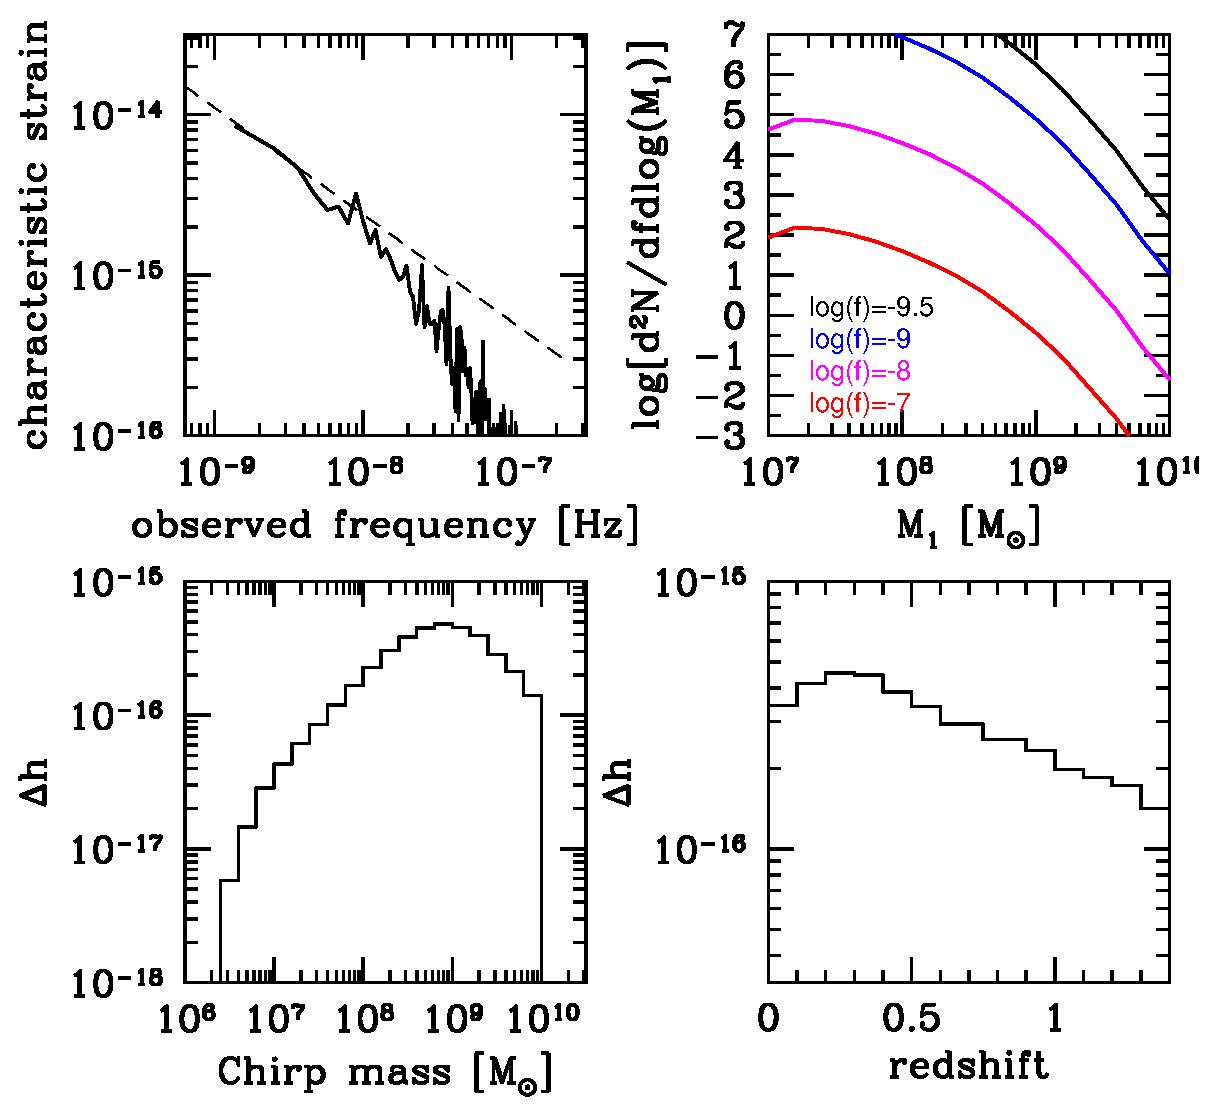
\includegraphics[width=8.0cm,clip=true,angle=0]{plots/fig_circ}&\hspace{1.0cm}
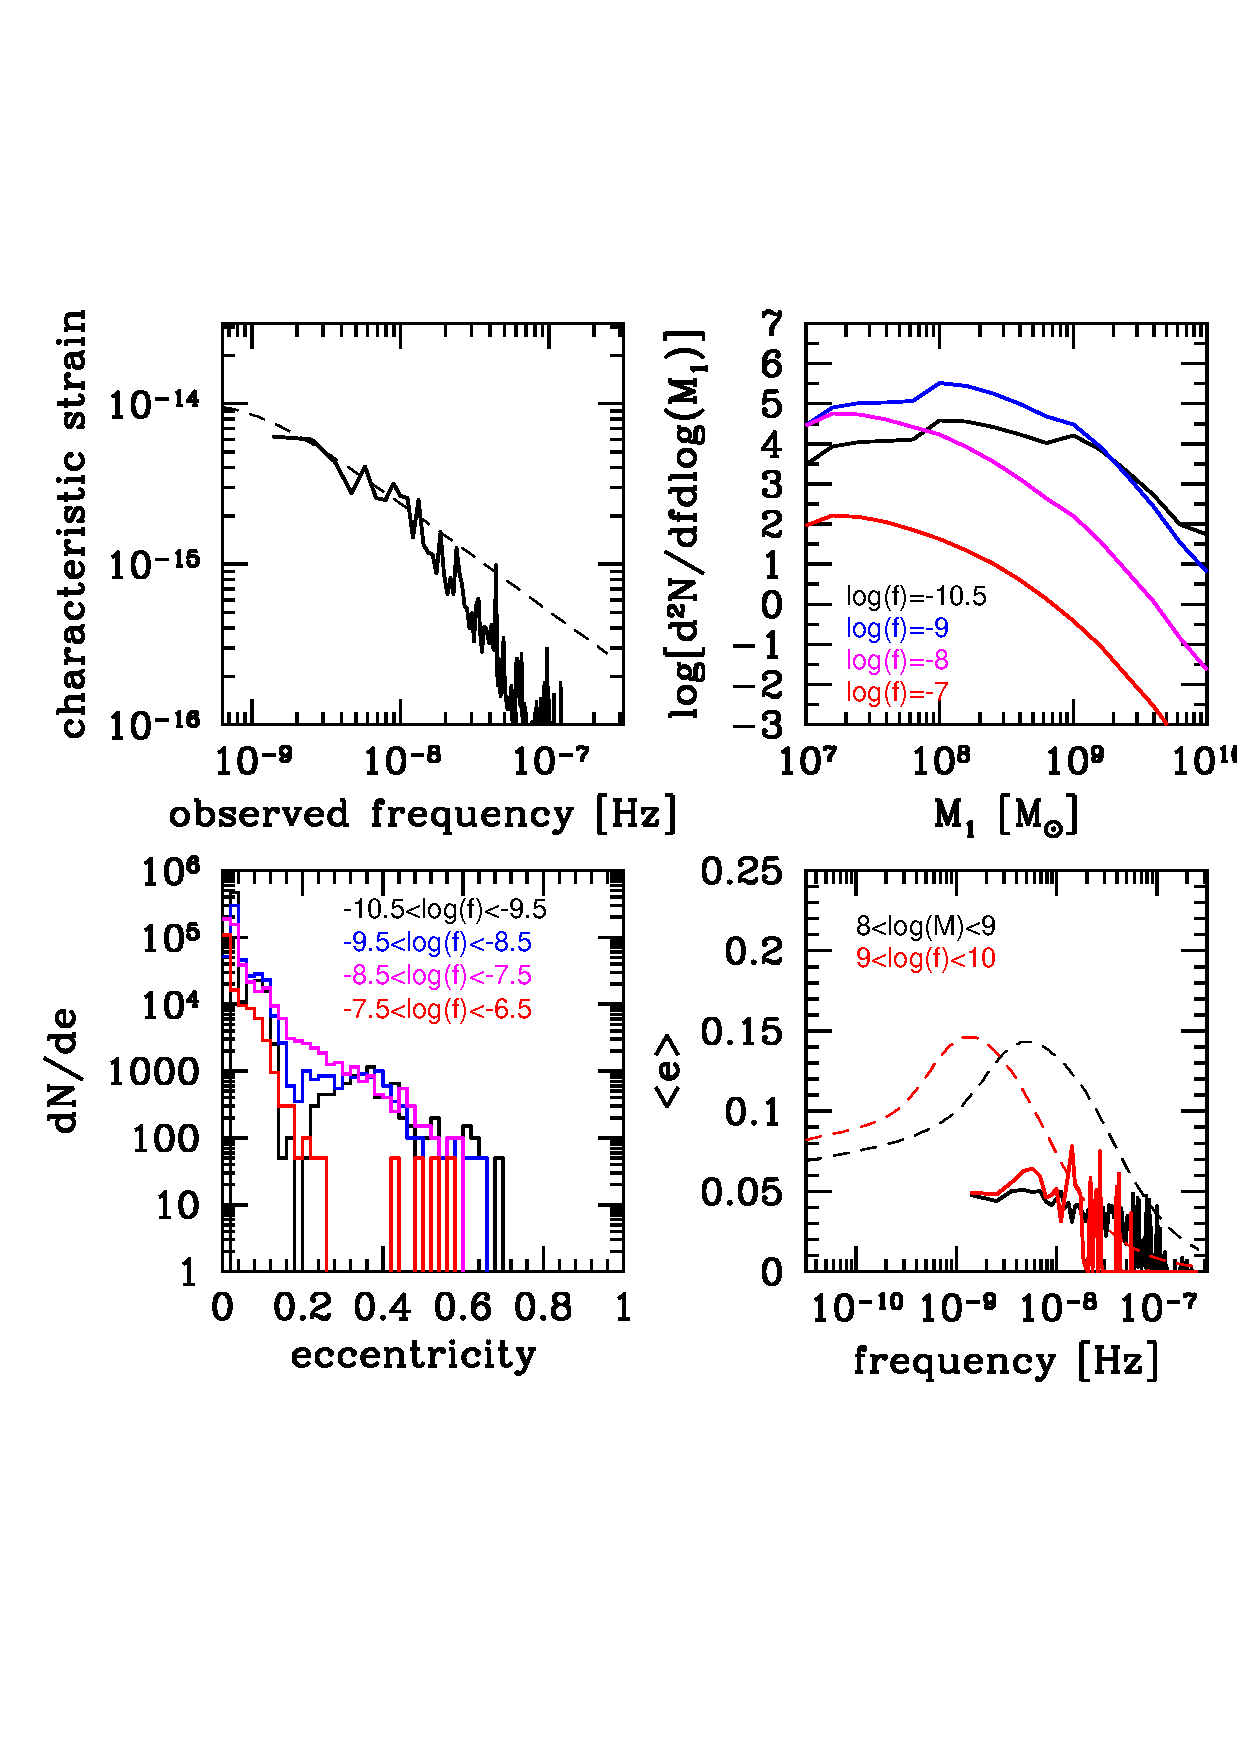
\includegraphics[width=8.0cm,clip=true,angle=0]{plots/fig_ecc0}\\
\vspace{0.7cm}\\
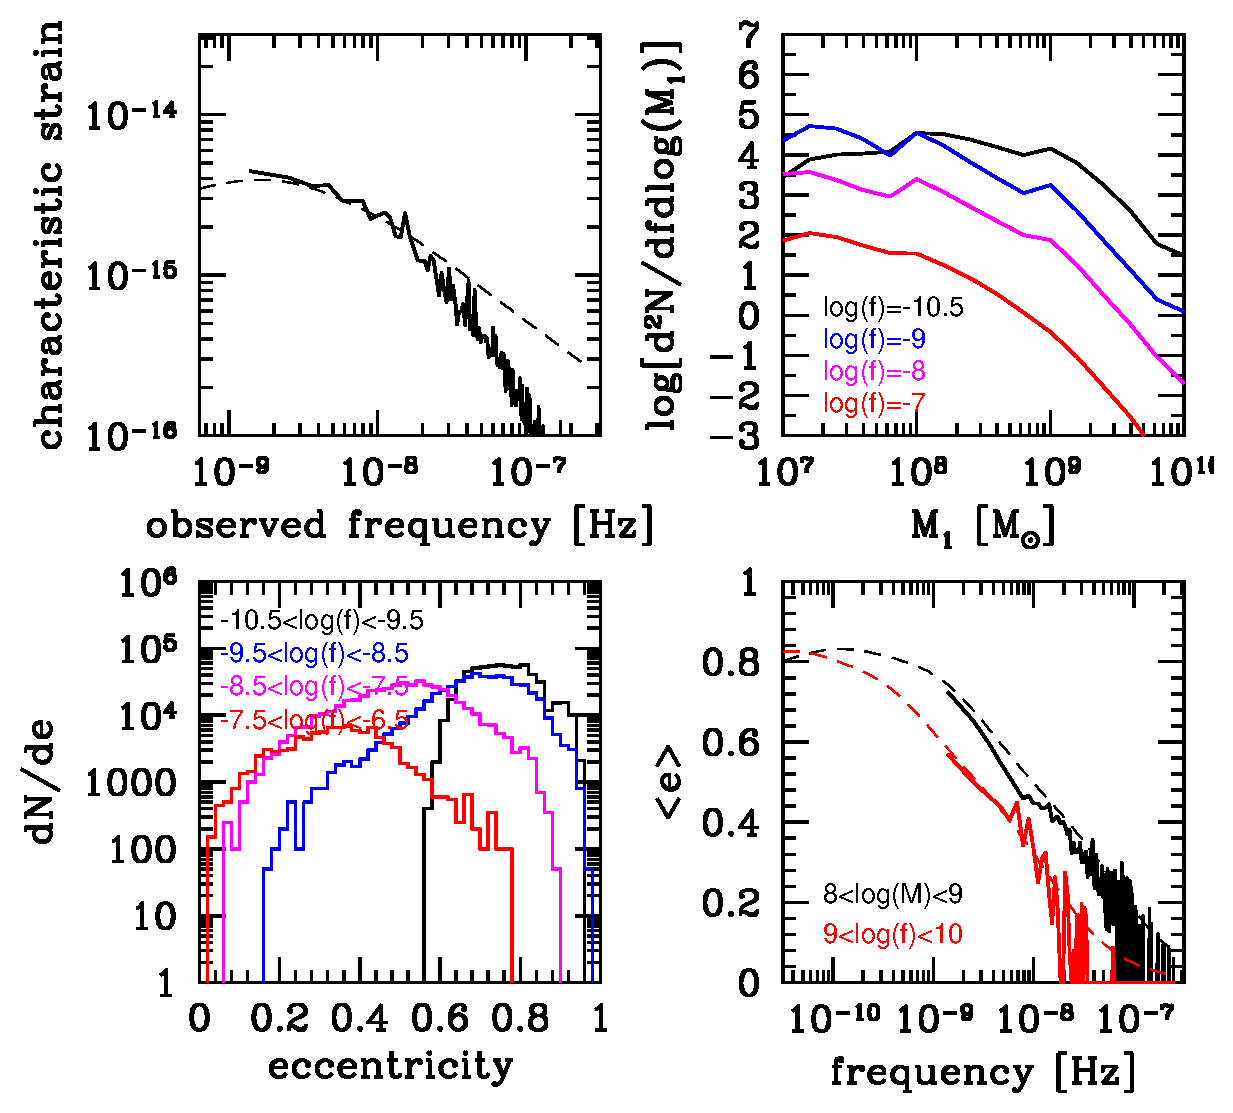
\includegraphics[width=8.0cm,clip=true,angle=0]{plots/fig_ecc5}&\hspace{1.0cm}
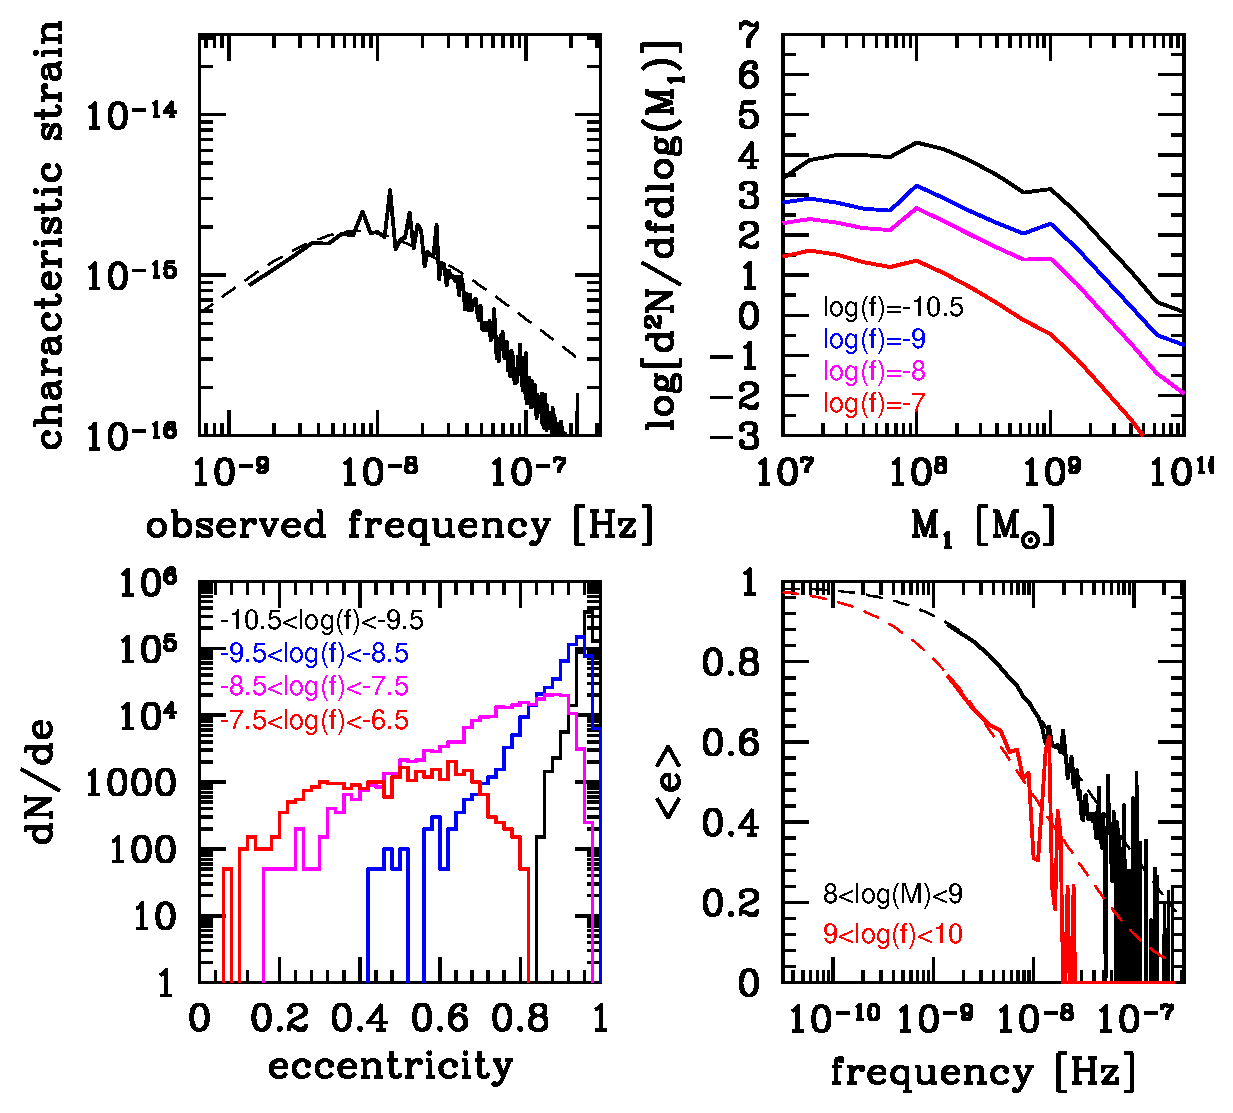
\includegraphics[width=8.0cm,clip=true,angle=0]{plots/fig_ecc9}\\
\end{tabular}
\caption{MBHB population models, described in the text. The four quadrants are for models  {\it pop\_circ} (top right), {\it pop\_e0} (top right), {\it pop\_e5} (bottom left), and {\it pop\_e9} (bottom right). Each quadrant is divided in four panels. In the top left and top right panel we show $h_c(f)$ and $d^2N/dfd{\rm log}M$ respectively. The two bottom panels show the contribution to the signal coming from different mass and redshift interval in the case of {\it pop\_circ} (top right quadrant); whereas for the other models, we show the behaviour of the eccentricity distribution of the population. (See main text for a more comprehensive description}.
\label{populations}
\end{figure*}
%%%%%%%%%%%%%%%%%%%%%%%%%%

\section{Circular Models for Michele}
I have also included 10 circular models in the folder {\it models\_for\_Michele}. Each folder contains 1000 files $MC\_SIM\_BKG\_1SU10YR\_*.out$. Each\begin{itemize}
\item Col 1: logarithm of the observed frequency in Hz;
\item Col 2: logarithm of $h_c$;
\item Col 3: nevermind.
\end{itemize}
The models span a factor of $\approx3$ in amplitude of the signal, and feature different prescriptions for building the MBHB merger rate (I can provide more details if needed). Michele can use the 1000 realization for each model to investigate the variance within a single model as a function of frequency.

There are also a bunch of other files in these directories, you can disregard those.

\end{document}

